A criação de uma \textit{\acrshort{api} Gateway} na \acrshort{clav} tem como objetivo principal contrariar o aumento da complexidade da \acrshort{api} de dados com a adição do controlo de acesso e da autenticação.

Para proceder à criação de uma \textit{\acrshort{api} Gateway} é importante primeiro entender o que é e quais os objetivos/aplicações de uma. Além disso, deve-se investigar as várias alternativas existentes no mercado e escolher aquela que melhor se adequa com os nossos requisitos. Na próxima secção são explorados estes pontos.

\section{Estado da Arte}

\subsection{\glsentryshort{api} Gateway}\label{sec:api_gateway}

Uma \textit{\acrshort{api} Gateway} encapsula a arquitetura interna em microserviços de uma aplicação, expondo uma única e simples \acrshort{api} através de um único \acrshort{url}, ou seja, um único ponto de entrada para a aplicação. Em arquiteturas baseadas em microserviços o não uso de uma \textit{\acrshort{api} Gateway} implica que os utilizadores da aplicação tenham provavelmente de agregar dados de diferentes serviços, manter vários \textit{endpoints}, realizar uma maior quantidade de pedidos e ter possivelmente uma autenticação diferente para cada serviço.

Uma \textit{\acrshort{api} Gateway} inclui normalmente~\cite{apiGatInfo,apiGatInfo2}:
\begin{itemize}
    \item Segurança (Autenticação e Autorização)
    \item Gestão de cotas e \textit{throttling}
    \item \textit{Caching}
    \item Processamento e composição da \acrshort{api}
    \item Roteamento
    \item Monitorização da \acrshort{api}
    \item Versionamento (possível automatização)
    \item Balanceamento de carga
    \item \textit{Rate Limit}
\end{itemize}

Além disso, a \textit{\acrshort{api} Gateway} tem como vantagens~\cite{apiGatInfo, apiGatInfo3}:
\begin{itemize}
    \item Simplifica o código da \acrshort{api};
    \item Oferece uma vista única e central da \acrshort{api} e, portanto, é mais provável que permita uma política consistente;
    \item A agregação e transformação de dados simplifica a interação dos clientes com os microserviços distribuídos. A agregação de dados permite também reduzir o número de pedidos;
    \item Esconde a arquitetura interna e distribui as aplicações baseadas em microserviços reduzindo, geralmente a sobrecarga de configuração;
    \item Código do cliente mais simples e limpo: quando os serviços cliente e \textit{backend} são separados, o cliente não necessita de saber os vários serviços individuais do \textit{backend} facilitando a manutenção do código bem como a reestruturação dos serviços sem que estas tenham impacto na interação entre cliente e \textit{backend}. Além disso, com uma \textit{\acrshort{api} Gateway} não é necessário construir lógica no cliente por forma a acompanhar os \textit{endpoints};
    \item Menos latência é igual a uma melhor experiência do utilizador: uma operação do lado do cliente pode necessitar de realizar vários pedidos aos serviços de \textit{backend}, aumentando a latência da operação. Com a presença de uma \textit{\acrshort{api} Gateway} pode ser efetuado um único pedido a esta que irá realizar os pedidos internos necessários, agregar os resultados e devolver a resposta ao cliente;
    \item Autenticação e Encriptação simplificada: Sem o uso de uma \textit{\acrshort{api} Gateway} cada serviço de \textit{backend} necessita de tomar as suas decisões de segurança o que aumenta a complexidade do código a desenvolver para um microserviço. Com o aumento da complexidade do código aumenta a possibilidade de erros bem como o aumento da superfície de ataque por utilizadores mal intencionados. Com o uso de uma \textit{\acrshort{api} Gateway} toda a segurança está centralizada num único serviço.
\end{itemize}

Contudo, tem como desvantagens~\cite{apiGatInfo}:
\begin{itemize}
    \item Possível ponto único de falha ou de \textit{bottleneck};
    \item Risco de complexidade já que todas as regras da \acrshort{api} estão num único local;
    \item Risco de \textit{lock-in} e a migração pode não ser simples.
\end{itemize}

Olhando um pouco mais da perspetiva da segurança, o controlo de acesso é a principal vantagem de segurança de uma \textit{\acrshort{api} Gateway} permitindo a uma organização gerir quem pode aceder à \acrshort{api} e estabelecer regras de como os pedidos de dados são tratados. O controlo de acesso estende-se também a outras políticas como o \textit{rate limit} às rotas da \acrshort{api} ou até o pagamento para aceder a certos recursos da \acrshort{api}.

Como todo o tráfego das rotas da \acrshort{api} passa por um \textit{gateway}, os especialistas de segurança sentem-se mais confiantes de que têm ``no pulso'' a \acrshort{api}.~\cite{apiGatInfo}

A \textit{\acrshort{api} Gateway} pode introduzir segurança nas mensagens enviadas entre os serviços internos através de encriptação tornando os serviços internos mais seguros. Além disso, é necessário um correto mecanismo de autenticação em conjunto com o uso de \acrshort{tls} por forma a evitar o acesso a rotas de pessoas não autorizadas. O uso de um mau mecanismo de autenticação (p.e. ser apenas necessário fornecer o número de telemóvel) pode levar a que qualquer pessoa consiga obter os dados de outra por exemplo.

Outro ponto a ter em conta em relação à proteção de uma \acrshort{api} é a proteção contra ameaças. Sem esta, a \textit{\acrshort{api} Gateway}, a(s) \acrshort{api}(s) e outros serviços estão inseguros. Ou seja, potenciais hackers ou \textit{malware} podem facilmente tentar propagar ataques tais como \acrshort{ddos} ou injeções de \acrshort{sql}, \textit{RegExp}, \acrshort{xml} ou ainda no caso específico da \acrshort{clav} injeções de \acrshort{sparql}. É assim importante realizar validação de \textit{input} da \acrshort{api}. 
As validações de \textit{input} mais comuns são:
\begin{itemize}
    \item Tamanho da mensagem;
    \item Proteção contra injeções \acrshort{sql};
    \item Proteção contra \textit{content-level attacks} do \acrshort{json}. Estes ataques são o uso de grandes ficheiros \acrshort{json} por forma a sobrecarregar o \acrshort{json} \textit{parser} e este eventualmente \textit{crashar};
    \item Proteção contra ameaças em \acrshort{xml}. Estes ataques envolvem normalmente \textit{payloads} recursivos, injeções \acrshort{sql} ou \textit{XPath}/\acrshort{xslt} com o mesmo intuito de sobrecarregar o \acrshort{xml} \textit{parser} e este eventualmente \textit{crashar}.
\end{itemize}

Já no caso do tratamento de erros e do código de estado \acrshort{http} em resposta aos pedidos, é uma boa prática que sejam devolvidos os códigos de estado corretos e com mensagens de erro curtas (apenas o necessário) sem incluírem o \textit{stack trace} visto ser um ponto de insegurança ao permitir qualquer intruso saber por exemplo, as \textit{packages} e as \textit{frameworks} usadas. A \textit{\acrshort{api} Gateway} pode ser usada para uniformizar as mensagens de erro devolvidas, impedindo também a possível exposição do código do \textit{backend}.

Por último, ao obrigar a autenticação de todos os utilizadores da \acrshort{api} e ao manter \textit{logs} dos acessos à \acrshort{api} torna possível limitar a taxa de consumo da \acrshort{api} para os utilizadores desta. Muitas \textit{\acrshort{api} Gateway}s permitem limitar o número de acessos que podem ser feitos para cada recurso da \acrshort{api} por segundo, minuto, dia ou outra restrição relevante.

Existem várias \textit{\acrshort{api} Gateway}s das quais se destacam \textit{Express Gateway}, \textit{Kong}, \textit{Moleculer \acrshort{api} Gateway}, \textit{Tyk \acrshort{api} Gateway} e \textit{Nginx Plus}. Iremos explorar um pouco de cada. Existem outras como, por exemplo, \textit{Amazon's \acrshort{api} Gateway}, contudo é apenas utilizável se pretendermos usar \acrshort{aws} e as suas máquinas para o \textit{deployment}. Como não é o caso, não a iremos explorar nesta secção.

\subsubsection{Express Gateway}

\textit{Express Gateway} é uma \textit{\acrshort{api} Gateway} que pode ser colocada em qualquer arquitetura de microserviços, independentemente da linguagem ou plataforma que se use. O \textit{Express Gateway} protege e expõe os microserviços através de \acrshort{api}s usando \textit{Node.js}, \textit{ExpressJS} e \textit{middleware} \textit{Express}. Além disso é \textit{open-source} e possui as seguintes funcionalidades~\cite{kong}:
\begin{itemize}
    \item Politicas empresariais que são normalmente pagas noutras \textit{\acrshort{api} Gateway}s são aqui gratuitas;
    \item Configuração através de um ficheiro \acrshort{yaml};
    \item Arquitetura de \textit{plugins};
    \item Extensível com mais de 3000 módulos;
    \item Corre em qualquer lado (\textit{Docker}, etc);
    \item Deteta automaticamente e recarrega quando há alterações na configuração;
    \item Suporta qualquer linguagem e \textit{framework};
    \item Suporta todos os casos de uso de microserviços, padrões e arquiteturas;
    \item Suporta \acrshort{https}, \acrshort{cors}, e \acrshort{jwt} entre outros.
\end{itemize}

Por definição, o \textit{Express Gateway} usa uma base de dados em memória para testes e para começar a experimentar. O \textit{Express Gateway} pode correr com ou sem \textit{backend} e se uma base de dados persistente for desejada é suportado o \textit{Redis}. A configuração do \textit{Express Gateway} é armazenada num ficheiro \acrshort{yaml} e como tal o \textit{Express Gateway} apenas guarda dados transacionais como informação de utilizadores e de \textit{tokens} de acesso na base de dados. Ou seja, nem sempre é necessário o uso da base de dados, depende do caso de uso.

A configuração como já referido é definida num ficheiro \acrshort{yaml} sendo que existe uma \acrshort{api} e uma \acrshort{cli} para gerir utilizadores e credenciais. Oficialmente não existe uma \acrshort{gui} para a \acrshort{api}.

Quanto ao desenvolvimento de \textit{plugins} para o \textit{Express Gateway} o mesmo pode ser feito através de \textit{JavaScript} usando a \textit{framework} \textit{Express}. Os \textit{plugins} são análogos ao \textit{middleware} \textit{Express}. 

\subsubsection{Kong}

O \textit{Kong} é uma \textit{\acrshort{api} Gateway} \textit{open-source} escalável, escrita em \textit{Lua} e que pode correr à frente de qualquer \acrshort{api}. O \textit{Kong} é construído em cima do \textit{Nginx}, \textit{OpenResty} e \textit{Apache Cassandra} ou \textit{PostgreSQL}. O \textit{core} do \textit{Kong} pode ser expandido em termos de funcionalidades e serviços através de \textit{plugins}.

Algumas das funcionalidades presentes são~\cite{kong}:
\begin{itemize}
    \item Tarefas de configuração e administração divididas entre \acrshort{rest} \acrshort{api} e \acrshort{cli};
    \item Extensível através de 36 \textit{plugins} disponíveis (6 deles são comerciais, o resto é \textit{open-source});
    \item Corre em qualquer lado (\textit{Kubernetes}, \textit{Docker}, etc);
    \item Escala ao apenas adicionar mais máquinas;
    \item Realiza balanceamento de carga dinamicamente através dos vários serviços de \textit{backend};
    \item Suporte para um conjunto de políticas para todos os \textit{endpoints} da \acrshort{api} que pode ser modificado com fluxo condicional;
    \item Suporta qualquer \textit{framework} e linguagem;
    \item Suporta todos os casos de uso de microserviços, padrões e arquiteturas;
    \item Suporta \acrshort{https}, \acrshort{cors}, e \acrshort{jwt} entre outros.
\end{itemize}

A forma mais fácil de instalar (\textit{deploy}) o \textit{Kong} é através do uso de \textit{Docker} ou de \textit{Kubernetes}.

A configuração do \textit{Kong} é armazenada no \textit{PostgreSQL} ou no \textit{Cassandra}. Há, contudo, a hipótese de usar uma configuração declarativa que não necessita de uma base de dados para manter a configuração. Esta configuração declarativa é definida pelo utilizador num ficheiro \acrshort{yaml} ou \acrshort{json} e tem várias vantagens já que reduz a carga de trabalho da máquina de instalação, reduz o número de dependências, diminui a necessidade de manutenção e permite a automatização do processo de \textit{deploy}.~\cite{KongDBLess} A \acrshort{gui} oficial de administração do \textit{Kong} apenas está disponível na versão paga, contudo é possível usar uma versão \textit{third-party} como por exemplo o \textit{Konga}.

Como o \textit{Kong} é construído sobre o \textit{Nginx} os vários \textit{plugins} necessitam de ser escritos em \textit{Lua}.

Uma das principais desvantagens do \textit{Kong} é que muitas das funcionalidades têm de ser ativadas através da configuração obrigando a um tempo inicial de \textit{setup}.

\subsubsection{Moleculer \glsentryshort{api} Gateway}

\textit{Moleculer} é uma \textit{framework} \textit{open-source} que contém as funcionalidades mais importantes numa arquitetura baseada em microserviços. Ajuda a construir serviços escaláveis, eficientes e fiáveis oferecendo também várias funcionalidades para construir e gerir os microserviços.

Das várias funcionalidades desta \textit{framework} está presente o módulo da \textit{\acrshort{api} Gateway}.

Esta \textit{\acrshort{api} Gateway} tem como funcionalidades~\cite{moleculerAPIG}:
\begin{itemize}
    \item Suporta \acrshort{http} e \acrshort{https};
    \item Serve ficheiros estáticos;
    \item Suporta \textit{middlewares};
    \item Suporta o \textit{upload} de ficheiros;
    \item Múltiplos \textit{body parsers} (\acrshort{json}, \textit{urlencoded});
    \item Cabeçalhos \acrshort{cors};
    \item \acrshort{http}2;
    \item \textit{Rate limiter};
    \item Suporta autorização;
    \item Modo \textit{middleware}.
\end{itemize}

Para além disso, esta \textit{\acrshort{api} Gateway} pode ser usada como \textit{middleware} numa \acrshort{api} desenvolvida com \textit{Express} (o caso da \acrshort{api} da \acrshort{clav}). Contudo, o recomendável para usar esta \textit{\acrshort{api} Gateway} é que a \acrshort{api} tenha sido desenvolvida com a \textit{framework} \textit{Moleculer}.

\subsubsection{Tyk \glsentryshort{api} Gateway}

O \textit{Tyk} é uma \textit{\acrshort{api} Gateway} \textit{open-source} com componentes gratuitos e outros pagos. Esta plataforma é escrita em \textit{Go} e é constituída por uma \textit{\acrshort{api} Gateway} e por um \textit{Dashboard}. Enquanto que o \textit{core} da \textit{\acrshort{api} Gateway} é gratuito e \textit{open-source}, o \textit{dashboard} requer a compra de licenças. A versão gratuita permite o uso de uma instância \textit{\acrshort{api} Gateway}. Para duas ou mais instâncias é necessário pagar. O \textit{Tyk} também possui uma versão \textit{cloud} (\textit{Tyk Cloud}) em que a versão gratuita permite até 50000 pedidos à \acrshort{api} diariamente. Acima deste limite é também necessário pagar.

Em termos de funcionalidades, o \textit{Tyk} possui~\cite{tyk}:
\begin{itemize}
    \item \acrshort{api} \acrshort{rest}ful;
    \item Múltiplos protocolos de acesso;
    \item \textit{Rate limiting} e cotas;
    \item Controlo de acesso granular;
    \item Expiração de chaves;
    \item Versionamento da \acrshort{api};
    \item \textit{Logs};
    \item \textit{Restarts} sem tempo de inatividade;
    \item Suporte para \acrshort{https}, \acrshort{cors}, \acrshort{jwt} entre outros.
\end{itemize}

O \textit{core} da \textit{\acrshort{api} Gateway} apenas necessita do \textit{Redis} contudo o produto todo (incluindo o \textit{dashboard}) necessita também, como dependências, do \textit{MongoDB} e do \textit{Tyk Pump}. 
Isto coloca uma maior carga na máquina do servidor que se pode evitar tornando também mais difícil de instalar e de gerir numa máquina local.

Em termos de administração, o \textit{Tyk} possui duas hipóteses, a gestão através da \textit{web} \acrshort{gui} ou através de \acrshort{rest} \acrshort{api}s. A configuração do \textit{Tyk} é armazenada no \textit{Redis}. O \textit{Tyk} é melhor que os seus concorrentes (\textit{Kong} e \textit{Nginx}) para projetos que pretendem ter a maioria das funcionalidades a funcionar desde o dia um (apenas na versão paga) visto não ser necessário explorar as várias opções disponíveis o que pode demorar algum tempo.~\cite{compAPIGat}

\subsubsection{Nginx Plus}

O \textit{Nginx Controller} disponível permite gerir o \textit{Nginx Plus} por forma a servir de \textit{load balancer}, \textit{proxy} ou ainda de \textit{\acrshort{api} Gateway}. Com o módulo \textit{\acrshort{api} Management} do \textit{Nginx Controller} é possível definir, publicar, proteger, monitorizar e analisar \acrshort{api}s. 
Para tal o \textit{Nginx Controller} gera a configuração para o \textit{Nginx Plus}.

Numa comparação de performance com o Kong verifica-se que o \textit{Nginx Plus} escala melhor do que o \textit{Kong}.~\cite{nginxPvsKong} Nos testes realizados chegou-se à conclusão que o módulo \textit{\acrshort{api} Management} do \textit{Nginx Plus} adiciona 20\% a 30\% menos latência aos pedidos dos utilizadores se compararmos com o \textit{Kong}. 
Além disso, usa menos 40\% de \acrshort{cpu} se compararmos com o \textit{Kong} para a mesma carga de trabalho.

Em termos de funcionalidades o \textit{\acrshort{api} Management} do \textit{Nginx Controller} possui~\cite{nginxP}:
\begin{itemize}
    \item Definição e publicação da \acrshort{api}: Permite criar múltiplas definições de \acrshort{api} e os seus recursos de componentes, gerir servidores \textit{backend}, direcionar recursos e publicar a configuração resultante nas instâncias \textit{Nginx Plus};
    \item \textit{Rate limiting}: Permite mitigar ataques de \acrshort{ddos} e protege as aplicações de serem inundadas de pedidos ao definir limites de \textit{bandwith} e de pedidos;
    \item \textit{Autenticação}: Permite autenticar pedidos usando \textit{\acrshort{api} keys} e \acrshort{jwt}s;
    \item Monitorização e alerta: Permite analisar a performance e as métricas das 
    instâncias \textit{Nginx Plus}. Permite também definir alertas quando alguma métrica ultrapassa certo valor.
\end{itemize}

Além destas funcionalidades é possível também usar o \textit{Nginx Controller} para criar/gerir \textit{load balancers}. 

O \textit{Nginx Plus} é uma versão paga e a versão gratuita do \textit{Nginx} não possui o \textit{Nginx Controller} mas é possível usar a versão gratuita através do uso de \textit{plugins} por forma a produzir uma \textit{\acrshort{api} Gateway}~\cite{compAPIGat}. 

O uso da versão gratuita obriga claro a um maior trabalho e a uma metodologia \textit{try and error} por forma a atingir o objetivo final.

A principal dificuldade na utilização do \textit{Nginx} é que a configuração pode ser um pouco complicada de usar e de perceber na sua totalidade possuindo uma acentuada curva de aprendizagem.

\section{Solução}

Nesta secção é escolhida a tecnologia \textit{\acrshort{api} Gateway} a usar de acordo com os requisitos necessários.

Apresentam-se de seguida os requisitos que a \textit{\acrshort{api} Gateway} deve possuir:
\begin{itemize}
    \item Ser gratuita e \textit{open-source};
    \item Suportar \acrshort{https}, \acrshort{cors} e \acrshort{jwt};
    \item Suportar Autenticação e Autorização personalizada (Criação de \textit{plugin}/middleware);
    \item Ser possível de automatizar ao definir apenas ficheiros de configuração sem qualquer uso de \acrshort{cli}s, 
    \acrshort{gui}s ou \acrshort{api}s;
    \item Suportar \textit{deployment} em \textit{Docker};
    \item Suportar \textit{rate limit} e \textit{cache};
    \item Suportar versionamento da \acrshort{api};
    \item Balancear carga e servir de \textit{reverse proxy};
    \item Gerar \textit{logs} e métricas;
    \item Ser capaz de integrar a documentação desenvolvida na especificação \textit{OpenAPI}.
\end{itemize}

Antes de fazer uma comparação entre as várias \textit{\acrshort{api} Gateway}s exploradas no estado de arte 
(~\ref{sec:api_gateway}) há uma que é imediatamente descartada, a \textit{Moleculer \acrshort{api} Gateway}. 
Esta \textit{\acrshort{api} Gateway} tem um melhor caso de uso quando a(s) \acrshort{api}(s) desenvolvida(s) 
usam a \textit{framework} \textit{Moleculer}. Como este não é o caso da \acrshort{clav} não teremos em consideração 
esta \textit{\acrshort{api} Gateway} na próxima tabela.

\begin{table}[H]
    \footnotesize
    \centering
    \begin{tabular}{|>{\centering\arraybackslash}p{0.3\textwidth}|>{\centering\arraybackslash}p{0.14\textwidth}|>{\centering\arraybackslash}p{0.14\textwidth}|>{\centering\arraybackslash}p{0.14\textwidth}|>{\centering\arraybackslash}p{0.14\textwidth}|}
    \hline
        Requisito & \textit{Nginx} & \textit{Kong} & \textit{Tyk} & \textit{Express Gateway} \\ \hline
        Ser gratuita e \textit{open-source} & {\color{green}\ding{52}} & {\color{green}\ding{52}} & {\color{green}\ding{52}} & {\color{green}\ding{52}} \\ \hline
        Suportar \acrshort{https}, \acrshort{cors} e \acrshort{jwt} & \acrshort{jwt} apenas na versão paga. Necessário usar \textit{plugin} & {\color{green}\ding{52}} & {\color{green}\ding{52}} & {\color{green}\ding{52}} \\ \hline
        Suportar Autenticação e Autorização personalizada (Criação de \textit{plugin}/middleware) & {\color{green}\ding{52}} (em \textit{Lua}) & {\color{green}\ding{52}} (em \textit{Lua} ou \textit{Go}) & {\color{green}\ding{52}} (em \textit{Python}, \textit{Lua} ou \textit{Javascript}) & {\color{green}\ding{52}} (em \textit{Javascript}) \\ \hline
        Ser possível de automatizar ao definir apenas ficheiros de configuração sem qualquer uso de \acrshort{cli}s, \acrshort{gui}s ou \acrshort{api}s & {\color{green}\ding{52}} & {\color{green}\ding{52}} & {\color{red}\ding{54}} & {\color{green}\ding{52}} \\ \hline
        Suportar deployment em \textit{Docker} & {\color{green}\ding{52}} & {\color{green}\ding{52}} & {\color{green}\ding{52}} & {\color{green}\ding{52}} \\ \hline
        Suportar \textit{rate limit} e \textit{cache} & {\color{green}\ding{52}} & {\color{green}\ding{52}} & {\color{green}\ding{52}} & Não possui \textit{cache} \\ \hline
        Suportar versionamento da \acrshort{api} & {\color{red}\ding{54}} & {\color{red}\ding{54}} & {\color{green}\ding{52}} & {\color{red}\ding{54}} \\ \hline
        Balancear carga e servir de \textit{reverse proxy} & {\color{green}\ding{52}} & {\color{green}\ding{52}} & {\color{green}\ding{52}} & {\color{green}\ding{52}} \\ \hline
        Gerar \textit{logs} e métricas & {\color{green}\ding{52}} & {\color{green}\ding{52}} & {\color{green}\ding{52}} & {\color{green}\ding{52}} \\ \hline
        Ser capaz de integrar a documentação desenvolvida na especificação \textit{OpenAPI} & {\color{red}\ding{54}} & {\color{red}\ding{54}} & {\color{green}\ding{52}} & {\color{red}\ding{54}} \\ \hline
    \end{tabular}
    \caption{Comparação entre \textit{\acrshort{api} Gateway}s~\cite{compAPIGat,kong,tyk}}
    \label{table:APIGateway}
\end{table}

Infelizmente nenhuma das tecnologias suporta todos os requisitos. 
Assim a partir da tabela~\ref{table:APIGateway} irá ser escolhida a tecnologia a usar tendo em conta a importância 
de cada requisito.

Das quatro tecnologias presentes na tabela, podemos desde já descartar o \textit{Tyk} visto não permitir 
automatizar o \textit{deployment}. Sobram, assim, o \textit{Nginx}, o \textit{Kong} e o \textit{Express Gateway}. 
Destas três, verifica-se que a última possui menos funcionalidades e portanto não será a tecnologia escolhida.

Entre o \textit{Nginx} e o \textit{Kong} a escolha irá prender-se com a facilidade e poder de configuração visto 
que os requisitos presentes em cada tecnologia são muito semelhantes. O \textit{Kong} é construído a partir do 
\textit{Nginx} (daí as suas parecenças em termos de requisitos presentes) e é possível configurar o 
\textit{Nginx} a partir do \textit{Kong}. Para além disso, o \textit{Kong} possui vários \textit{plugins} por 
forma a permitir certas funcionalidades que no \textit{Nginx} seria necessário configurar manualmente. Portanto a escolha tecnológica para a \textit{\acrshort{api} Gateway} recai 
sobre o \textit{Kong}.

\subsection{Arquitetura}

Após a escolha da \textit{\acrshort{api} Gateway} a usar (\textit{Kong}) é necessário proceder ao esboço de 
uma arquitetura base a desenvolver. Esta arquitetura apresenta-se de seguida, na figura~\ref{fig:apiGatewayArch}, onde apenas se inclui a 
\acrshort{api} visto a interface não sofrer qualquer alteração:
\begin{figure}[H]
    \centering
    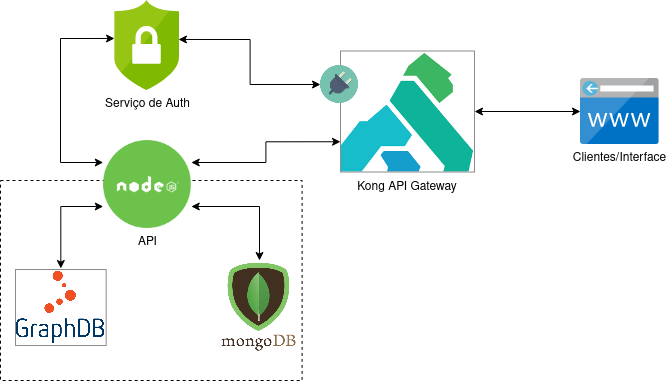
\includegraphics[width=1\textwidth]{img/apiGatewayArch.png}
    \caption{Arquitetura a desenvolver com \textit{\acrshort{api} Gateway}}\label{fig:apiGatewayArch}
\end{figure}

Apesar das várias vantagens do \textit{Kong} não é possível, através dos \textit{plugins} fornecidos por este, 
realizar uma proteção das rotas semelhante à presente na \acrshort{api} de dados da \acrshort{clav}. 
Portanto, com o intuito de simplificar a \acrshort{api} de dados, a ideia passa por retirar da \acrshort{api} de 
dados da \acrshort{clav} tudo que envolva a proteção desta, tais como a verificação de \textit{tokens} (autenticação), 
a geração de \textit{tokens} bem como a verificação da autorização de um utilizador (verificar se o nível do 
utilizador é suficiente para aceder determinada rota), e colocar estas funcionalidades noutro servidor 
independente da \acrshort{api} de dados. Este servidor está representado na arquitetura como Serviço de 
\textit{Auth} e procederá então à autenticação e autorização dos pedidos realizados pelos clientes.

Com esta separação a \acrshort{api} de dados precisará de realizar pedidos ao Serviço de \textit{Auth} para a 
verificação e geração de \textit{tokens} em casos particulares como o \textit{login} de um utilizador ou a 
\textit{criação} de uma Chave \acrshort{api}.

Todos os pedidos realizados pelos clientes e pela interface da \acrshort{clav} têm como ponto de entrada o 
\textit{Kong}. Este, através de um \textit{plugin}, para cada pedido recebido irá realizar um pedido ao Serviço 
de \textit{Auth} onde:

\begin{enumerate}
    \item Verifica quem pode aceder (que tipo de clientes) à rota do pedido;
    \item Procede à autenticação do pedido (se necessário);
    \item Procede à autorização do pedido (se necessário).
\end{enumerate}

Caso a resposta do Serviço de \textit{Auth} seja positiva então o \textit{Kong} procederá à realização do pedido 
à \acrshort{api} de dados. Caso contrário, o pedido à \acrshort{api} de dados não é efetuado e é devolvida à máquina cliente 
uma resposta com o erro correspondente (erro de autenticação ou de autorização).

\section{Implementação}

Nesta secção irá ser abordada a configuração do \textit{Kong} além do desenvolvimento do Serviço de \textit{Auth} adicional para a proteção da \acrshort{api} de dados.

\subsection{Serviço de \textit{Auth}}
Este serviço, desenvolvido em \textit{Node.js}, tem como principal papel a autenticação e autorização dos pedidos recebidos na plataforma \acrshort{clav}. Além disso, este serviço irá tratar de verificar e gerar \textit{tokens} (\acrshort{jwt}s). 

Para saber quem pode aceder determinada rota, o Serviço de \textit{Auth} possui um dicionário em que cada chave é um verbo \acrshort{http} e em cada verbo existe um dicionário com os vários caminhos desse verbo. A cada caminho é associado um valor que indica quem pode aceder a rota. Este valor é:
\begin{itemize}
    \item \textbf{-1:} Todos podem aceder
    \item \textbf{0:} Só podem aceder Chaves API autenticadas ou utilizadores autenticados
    \item \textbf{Um número maior que 0:} Só podem aceder utilizadores autenticados com nível igual ou superior ao número
    \item \textbf{Lista de números maiores que 0:} Só podem aceder utilizadores autenticados com nível presente nesta lista
\end{itemize}
A ordem dos caminhos em cada verbo é importante visto que as rotas são testadas por ordem e, quando há um \textit{match}, é assumido que é essa a rota do pedido não sendo testado o resto dos caminhos.

Consoante o valor obtido do dicionário é feita a autenticação e autorização necessária para a rota. Caso não seja obtido um valor, assume-se que a rota não existe na \acrshort{api} de dados.

Sempre que for acrescentada uma nova rota na \acrshort{api} de dados é necessário adicionar essa neste dicionário com as devidas permissões.

Este serviço de autenticação e autorização disponibiliza cinco rotas:
\begin{description}
    \item[POST /auth] Autenticar e Autorizar um pedido. Recebe no \textit{body} o verbo, o caminho, a \textit{query string} e os cabeçalhos do pedido a efetuar para a \acrshort{api} de dados. Como resposta devolve respostas com \textit{\acrshort{http} status}:
    \begin{itemize}
        \item 200: o pedido pode ser efetuado à \acrshort{api} de dados. Esta resposta possui no \textit{body} a informação contida no \textit{token} se este for enviado no pedido;
        \item 401: \textit{token} inválido ou pedido sem autenticação para aceder a rota;
        \item 403: pedido sem autorização para aceder a rota;
        \item 404: a rota não existe.
    \end{itemize}
    \item[POST /user/sign] Gerar um \textit{token} para um utilizador. Recebe no \textit{body} do pedido a informação do utilizador e o tempo de expiração a usar para o \textit{token}. Como resposta devolve o \textit{token} gerado;
    \item[POST /user/verify] Verificar um \textit{token} de um utilizador. Recebe no \textit{body} o \textit{token} do utilizador. Como resposta, caso o \textit{token} seja válido, devolve a informação contida no \textit{token};
    \item[POST /apikey/sign] Gerar um \textit{token} para uma Chave API. Recebe no \textit{body} do pedido a informação da Chave API e o tempo de expiração a usar para o \textit{token}. Como resposta devolve o \textit{token} gerado;
    \item[POST /apikey/verify] Verificar um \textit{token} de uma Chave API. Recebe no \textit{body} o \textit{token} da Chave API. Como resposta, caso o \textit{token} seja válido, devolve a informação contida no \textit{token}.
\end{description}

Nenhuma destas rotas está disponível externamente, ou seja, é apenas acessível pelo \textit{Kong} e pela \acrshort{api} de dados.

A necessidade de rotas diferentes para utilizadores e Chaves API deve-se ao facto de serem usados pares de chave pública/privada diferentes para gerar e verificar os \textit{tokens}. Para esta geração e verificação é usada a mesma biblioteca usada até agora, \texttt{jsonwebtoken}. Continua-se também a usar os extratores da biblioteca \textit{passport-jwt} para obter os \textit{tokens} dos pedidos, mas já não se recorre ao \textit{passport} para proceder à autenticação visto não ser necessário.

Com a existência deste serviço, a \acrshort{api} de dados sem \textit{Kong} deixou de estar protegida e nos casos em que necessita, de forma excecional, de verificar ou a gerar  \textit{tokens} recorre à \acrshort{api} do Serviço de \textit{Auth}. Apesar disso continua a ser essencial que a \acrshort{api} de dados saiba quem realizou o pedido. Essa informação será enviada num cabeçalho pelo \textit{Kong} algo que será explicado na próxima secção. Ou seja, o serviço de \textit{Auth} não é apenas um \textit{middleware} na \textit{pipeline} do \textit{Kong} mas um serviço na rede de microserviços da plataforma \acrshort{clav}.

\subsection{\textit{Plugin} \texttt{external-auth}}
Como já referido anteriormente não é possível, usando os \textit{plugins} disponíveis do \textit{Kong}, obter uma proteção semelhante à presente na \acrshort{api} de dados. Para resolver esta situação havia duas hipóteses, criar um \textit{plugin} que tratasse da autenticação e da autorização ou criar um \textit{plugin} que intercetasse os pedidos, realizasse um pedido a um serviço externo para tratar da autenticação e da autorização, e consoante a resposta deixasse ou não o pedido ser realizado. A segunda hipótese foi a escolhida visto que implica a criação de um \textit{plugin} de menores dimensões, que tem de ser desenvolvido em \textit{Lua}, e permite por outro lado aproveitar parte do código de autenticação e autorização presente na \acrshort{api} de dados e usá-lo no serviço externo. Ou seja, é uma abordagem mais rápida e simples para além de que este \textit{plugin} de menores dimensões encontrava-se já em parte desenvolvido\footnote{Ver \url{https://github.com/aunkenlabs/kong-external-auth}} onde foi apenas necessário realizar algumas melhorias como a possibilidade de devolver respostas 403 e 404 entre outras alterações\footnote{Ver \url{https://github.com/jcm300/kong-external-auth}}.

De uma forma mais pormenorizada, quando um pedido é recebido pelo \textit{Kong}, este pedido poderá passar por vários \textit{plugins} de acordo com a configuração usada antes e após ser efetuado o pedido à \acrshort{api} de dados. O \textit{plugin} \texttt{external-auth} se adicionado na configuração é executado antes do pedido ser efetuado à \acrshort{api} de dados. Este \textit{plugin} obtém do pedido o caminho, o verbo, a \textit{query string} e os cabeçalhos e envia-os no \textit{body} dum pedido que faz ao serviço externo. Quando o \textit{plugin} recebe a resposta do serviço externo, consoante o \textit{\acrshort{http} status} da resposta, irá ter a seguinte reação:
\begin{itemize}
    \item 200: Insere no pedido a efetuar à \acrshort{api} de dados o cabeçalho \texttt{CLAV-Auth} onde é enviada em formato \textit{string} a resposta do serviço externo;
    \item 401: Devolve uma resposta de erro para o utilizador com \textit{\acrshort{http} status} 401;
    \item 403: Devolve uma resposta de erro para o utilizador com \textit{\acrshort{http} status} 403;
    \item 404: Devolve uma resposta de erro para o utilizador com \textit{\acrshort{http} status} 404;
    \item Restantes: Devolve uma resposta de erro para o utilizador com \textit{\acrshort{http} status} 401.

\end{itemize}

Portanto quando um pedido possui autenticação e autorização pelo serviço externo, este pedido inclui também um cabeçalho \texttt{CLAV-Auth} onde estará presente a informação presente no \textit{token}, seja de um utilizador ou de uma Chave API. Este cabeçalho será interpretado pela \acrshort{api} de dados por forma a esta saber quem realizou o pedido. No caso do cabeçalho não ser enviado, for vazio ou num formato incorreto, a \acrshort{api} de dados irá considerar que o pedido foi efetuado por alguém ``Desconhecido''.

Este \textit{plugin} está disponível em \url{https://luarocks.org/modules/jcm300/external-auth}.

\subsection{Configuração \textit{Kong}}
O \textit{Kong} pode ser configurado através de um ficheiro de configuração \texttt{.conf} onde é definido o modo em que executa, possíveis ligações a bases de dados, configurações do \textit{Nginx}, entre outros. Contudo não é neste ficheiro que se define o comportamento que o \textit{Kong} efetua quando recebe determinado pedido, apesar de se poder alterar algum comportamento através de configurações do \textit{Nginx}. Para definir o comportamento do \textit{Kong} há três hipóteses. A que foi escolhida, configuração declarativa, permite que o \textit{Kong} execute sem necessitar de uma base de dados para armazenar as configurações visto que as configurações são definidas num ficheiro \acrshort{yaml} ou \acrshort{json} que é carregado para memória. Assim não se sobrecarrega desnecessariamente o servidor que executa o \textit{Kong}.

Para usar esta configuração declarativa é necessário no ficheiro de configuração \texttt{.conf} colocar a diretiva \texttt{database} com o valor \texttt{off} e a diretiva \texttt{declarative\_config} com o caminho do ficheiro da configuração declarativa.

Na configuração declarativa são usados vários \textit{plugins} a maioria desenvolvidos pelo \textit{Kong} exceto o \textit{external-auth}. 

Por predefinição os \textit{plugins} do \textit{Kong} estão disponíveis. Para se puder usar \textit{plugins} externos é necessário indicá-los no ficheiro \textit{.conf} na diretiva \texttt{plugins}. Assim o valor aqui colocado foi \texttt{blunded,external-auth} indicando que se pretende usar os \textit{plugins} do \textit{Kong} (\texttt{blunded}) e o \textit{external-auth}. 

Antes de iniciar o \textit{Kong} será depois necessário instalar o \textit{plugin} \textit{external-auth}. 

No ficheiro \textit{.conf} é também indicado para onde os logs de erro e acesso são enviados sendo os de erro enviados para o \texttt{stderr} e os de acesso para o \texttt{stdout}. Além disso indica-se também em que portas (\acrshort{http} e \acrshort{https}) o \textit{Kong} irá receber os pedidos bem como em que portas está acessível a \acrshort{api} de administrador (como é usada uma configuração declarativa esta \acrshort{api} será apenas de leitura).

O primeiro passo na configuração declarativa foi adicionar o serviço da \acrshort{api} de dados e associar desde logo o \textit{plugin} necessário para a proteção da \acrshort{api} de dados:
\begin{lstlisting}[language=yaml, caption=Configuração declarativa do \textit{Kong}: \acrshort{api} de dados]
services:
  - name: API
    url: ${API_HOST}
    routes:
      - name: TodasRotas
        paths:
          - /
    plugins:
      - name: external-auth
        config:
          url: ${SERVER_AUTH_HOST}
          path: /auth
\end{lstlisting}

Com esta configuração inicial o \textit{Kong} reencaminha todos os pedidos que comecem por \texttt{/} para a \acrshort{api} de dados, usando neste serviço o \textit{plugin} \texttt{external-auth} já descrito. Temos assim uma primeira versão funcional com autenticação e autorização da \acrshort{api} de dados.

Contudo a \acrshort{api} de dados necessita de permitir \acrshort{cors} e para tal é adicionado o \textit{plugin} do \textit{Kong} chamado \texttt{cors}\cite{kongCORS}:
\begin{lstlisting}[language=yaml, caption=Configuração declarativa do \textit{Kong}: \textit{plugin} \texttt{cors}]
services:
  - name: API
    ...
    plugins:
      ...
      - name: cors
        service: API
        config:
          origins:
            - '*'
          methods:
            - GET
            ...
          headers:
            - Accept
            ...
          credentials: true
\end{lstlisting}

Além deste foram adicionados mais 3 \textit{plugins} do \textit{Kong} a este serviço, cada um com objetivos diferentes. 

O \textit{plugin} \texttt{rate-limiting} por forma a limitar o número de pedidos efetuados a 10 pedidos por segundo por endereço \acrshort{ip}\cite{kongRateLimiting}:
\begin{lstlisting}[language=yaml, caption=Configuração declarativa do \textit{Kong}: \textit{plugin} \texttt{rate-limiting}]
services:
  - name: API
    ...
    plugins:
      ...
      - name: rate-limiting
        config:
          second: 10
          policy: local
\end{lstlisting}

É possível também aplicar este \textit{plugin} a rotas especificas da \acrshort{api} de dados.

Por outro lado, o \textit{plugin} \texttt{proxy-cache} é usado para realizar a \textit{cache} de respostas de pedidos \texttt{text/plain} (texto) ou \texttt{application/json} (\acrshort{json}) com verbos \texttt{GET} e \texttt{HEAD} e \textit{\acrshort{http} status} 200, 301 e 404 por uma hora\cite{kongProxyCache}:

\begin{lstlisting}[language=yaml, caption=Configuração declarativa do \textit{Kong}: \textit{plugin} \texttt{proxy-cache}]
services:
  - name: API
    ...
    plugins:
      ...
      - name: proxy-cache
        config:
          cache_ttl: 3600 #segundos (1h) em cache
          strategy: memory
\end{lstlisting}

Com este \textit{plugin} é possível evitar pedidos recentes à \acrshort{api} de dados iguais bem como acelerar o tempo de resposta dos pedidos que foram recentemente efetuados.

É ainda usado o \textit{plugin} \texttt{response-transformer} por forma a adicionar cabeçalhos na resposta devolvida pela \acrshort{api} de dados. Estes cabeçalhos têm como objetivo melhorar a segurança da \acrshort{api} e cumprir algumas das recomendações de segurança \acrshort{https} já referidas em~\ref{sec:sol_httpsReq}~\cite{kongResponseTransformer}:

\begin{lstlisting}[language=yaml, caption=Configuração declarativa do \textit{Kong}: \textit{plugin} \texttt{response-transformer}]
services:
  - name: API
    ...
    plugins:
      ...
      - name: response-transformer
        config:
          remove:
            headers:
              - strict-transport-security
              ...
              - content-security-policy
          add:
            headers:
              - 'Strict-Transport-Security: max-age=31536000; includeSubDomains; preload'
              ...
              - "Content-Security-Policy: default-src 'none'"
\end{lstlisting}

Este \textit{plugin} possui a seguinte ordem de execução: remover (\textit{remove}), renomear (\textit{rename}), substituir (\textit{replace}), adicionar (\textit{add}) e acrescentar (\textit{append}).

A adição dos \textit{plugins} (\texttt{cors} e \texttt{response-transformer}) permite assim a remoção da \acrshort{api} de dados das bibliotecas \texttt{cors} e \texttt{helmet} que eram usadas para alcançar os mesmos objetivos para os quais estes \textit{plugins} vão ser usados.

A adição do cabeçalho \texttt{Content-Security-Policy} com o valor \texttt{default-src 'none'} no \textit{plugin} \texttt{response-transformer} impede qualquer conteúdo que não a resposta em si. Contudo a \acrshort{api} de dados possui uma página de documentação na rota \texttt{/<Versão da API>/docs} que irá necessitar de um \texttt{Content-Security-Policy} diferente. 

Para tal, definiu-se uma rota na configuração declarativa associando-a ao serviço da \acrshort{api} de dados mas no qual o \textit{plugin} \texttt{response-tranformer} possui um valor diferente para o cabeçalho \texttt{Content-Security-Policy}. Os outros \textit{plugins} associados ao serviço da \acrshort{api} de dados continuam a ser executados para esta rota mas o \textit{plugin} \texttt{response-tranformer} desse serviço é substituído por este definido na rota:

\begin{lstlisting}[language=yaml, caption=Configuração declarativa do \textit{Kong}: Rota da documentação]
routes:
  - name: docs
    service: API
    strip_path: false
    paths:
      - /$API_VERSION/docs
    methods:
      - GET
    plugins:
      - name: response-transformer
        config:
          remove:
            headers:
              - strict-transport-security
              ...
              - content-security-policy
          add:
            headers:
              - 'Strict-Transport-Security: max-age=31536000; includeSubDomains; preload'
              ...
              - "Content-Security-Policy: default-src 'self' $DOMAINS; img-src 'self' https://validator.swagger.io data: $DOMAINS; style-src 'self' 'unsafe-inline' $DOMAINS; script-src 'self' 'unsafe-inline' $DOMAINS"
\end{lstlisting}

A propriedade \texttt{strip\_path} com valor falso impede que o \textit{Kong} associe (parecido com um \textit{bind}) o caminho \texttt{/<Versão API>/docs} do \textit{Kong} ao caminho \texttt{/} da \acrshort{api} de dados. Assim, quando se faz o pedido a esta rota o pedido que é feito na \acrshort{api} de dados é no caminho \texttt{/<Versão API>/docs} desta. 
Por fim, procedeu-se à configuração do \acrshort{https} no \textit{Kong}. Como se usam os certificados do \textit{Let's Encrpyt} pode-se usar o \textit{plugin} \texttt{acme} do \textit{Kong}\cite{kongACME}:

\begin{lstlisting}[language=yaml, caption=Configuração declarativa do \textit{Kong}: \textit{plugin} \texttt{acme}]
plugins:
  - name: acme
    config:
      account_email: $EMAIL
      domains: $DOMAINS_LIST
      renew_threshold_days: 30
      storage: redis
      storage_config:
        redis:
          auth: "redisPass123"
          port: 6379
          database: 0
          host: $REDIS_HOST
      tos_accepted: true
\end{lstlisting}

Para manter a configuração e os certificados do \textit{plugin} após reinícios do \textit{Kong} usa-se o \textit{Redis} para guardar a configuração bem como os certificados. Convém referir que este \textit{plugin} tem de ser global na configuração declarativa e não associado a um único serviço. Além disso, para permitir a geração dos certificados pelo \textit{Let's Encrypt} é necessário permitir o acesso à rota que começa em \texttt{/.well-known/acme-challenge} para permitir a validação do controlo do domínio. Assim foi adicionado o seguinte serviço à configuração declarativa:

\begin{lstlisting}[language=yaml, caption=Configuração declarativa do \textit{Kong}: Serviço para a geração de certificados \acrshort{tls}]
services:
  - name: acme-dummy
    url: http://127.0.0.1:65535
    routes:
      - name: acme-dummy
        paths:
          - /.well-known/acme-challenge
  - name: API
    ...
\end{lstlisting}

Para ativar também o uso do \textit{plugin} \texttt{acme} é necessário no ficheiro \texttt{.conf} indicar onde estão os certificados confiáveis por forma a ser possível o \textit{Kong} iniciar para depois puder obter os certificados do \textit{Let's Encrypt}. Para tal, é indicado na diretiva \texttt{nginx\_proxy\_lua\_ssl\_trusted\_certificate} o valor \texttt{/etc/ssl/certs/ca-certificates.crt} (esta é a localização no caso de uma distribuição \textit{Ubuntu}, poderá ser diferente noutras distribuições e \acrshort{os}'s). Quando o \textit{Kong} iniciar para acionar a criação do certificado é necessário fazer um pedido ao \textit{Kong} correndo o seguinte comando:

\begin{lstlisting}[language=bash]
curl https://<domain> -k
\end{lstlisting}

substituindo \verb|<domain>| pelo domínio da \acrshort{api} de dados.

Além disso, por forma a que quando alguém tente aceder às rotas através de \acrshort{http} seja redirecionado para o \acrshort{https} foram adicionadas as seguintes propriedades nas rotas:

\begin{lstlisting}[language=yaml, caption=Configuração declarativa do \textit{Kong}: Serviço para a geração de certificados \acrshort{tls}]
services:
  ...
  - name: API
    ...
    routes:
      - name: TodasRotas
        protocols:
          - https
        https_redirect_status_code: 301
        ...
    ...

routes:
  - name: docs
    ...
    protocols:
      - https
    https_redirect_status_code: 301
    ...
\end{lstlisting}

A propriedade \texttt{protocols} indica que protocolos deverão estar disponíveis na rota e a propriedade \texttt{https\_redirect\_status\_code} indica o \textit{status code} nos casos em que os pedidos são efetuados para o \acrshort{http}. Como este \textit{status code} é 301 os clientes serão redirecionados para o \acrshort{https}.

Por fim, por forma a melhorar a segurança do \acrshort{https} e cumprir as recomendações de segurança são adicionadas no ficheiro de configuração \texttt{.conf} algumas diretivas de configuração do \textit{Nginx}:

\begin{lstlisting}[caption=Configurações do \textit{Nginx} no ficheiro de configuração \texttt{.conf}]
#Indicar que se pretende usar ciphers personalizados
ssl_cipher_suite = custom
#Ciphers permitidos a usar por ordem de preferência
sel_ciphers = EECDH+AESGCM:EDH+AESGCM:ECDHE-RSA-AES128-GCM-SHA256:AES256+EECDH:DHE-RSA-AES128-GCM-SHA256:AES256+EDH:ECDHE-RSA-AES256-GCM-SHA384:DHE-RSA-AES256-GCM-SHA384:ECDHE-RSA-AES256-SHA384:ECDHE-RSA-AES128-SHA256:ECDHE-RSA-AES256-SHA:ECDHE-RSA-AES128-SHA:DHE-RSA-AES256-SHA256:DHE-RSA-AES128-SHA256:DHE-RSA-AES256-SHA:DHE-RSA-AES128-SHA:ECDHE-RSA-DES-CBC3-SHA:EDH-RSA-DES-CBC3-SHA:AES256-GCM-SHA384:AES128-GCM-SHA256:AES256-SHA256:AES128-SHA256:AES256-SHA:AES128-SHA:DES-CBC3-SHA:HIGH:!aNULL:!eNULL:!EXPORT:!DES:!MD5:!PSK:!RC4

#Protocolos SSL permitidos
nginx_http_ssl_protocols = TLSv1.2 TLSv1.3
#Indicar que se deve preferir os ciphers do servidor em vez do cliente
nginx_http_ssl_prefer_server_ciphers = on

#DH parameters mais forte
nginx_http_ssl_dhparam = /etc/ssl/certs/dhparam.pem

#Especifica a curva a usar para os ciphers ECDHE
nginx_http_ssl_ecdh_curve = secp384r1

#Ativar stapling, infelizmente não funciona porque o plugin acme usado ainda não suporta
nginx_http_ssl_stapling = on
nginx_http_ssl_stapling_verify = on

#Melhorar tolerância quando o endereço de um dominio muda
nginx_http_resolver = 8.8.8.8 8.8.4.4 valid=300s
nginx_http_resolver_timeout = 5s

#Tempo em que pode ser reusada uma sessão
nginx_http_ssl_session_timeout = 1d

#Tempo em que é mantida uma conexão idle a um servidor
nginx_upstream_keepalive_timeout = 65
\end{lstlisting}

Uma pequena nota. As variáveis ambiente (\verb|${var}| ou \verb|$var|) serão substituídas antes de serem usadas pelo \textit{Kong} ao aplicar o comando \texttt{envsubst} ao ficheiro da configuração declarativa.

Convém também referir que, esta versão da \acrshort{api} de dados com \textit{Kong} respeita todos os requisitos enunciados na migração de \acrshort{http} para \acrshort{https} (\ref{sec:sol_httpsReq}) com o objetivo primordial de melhorar a segurança. Para o \textit{deployment} foi também usado o \textit{docker} e o \textit{docker-compose} o que é descrito na secção~\ref{sec:deployKong}.

\subsection{Arquitetura}
Na figura~\ref{fig:apiGatewayArch} apresentou-se uma visão inicial da arquitetura. Já na figura~\ref{fig:apiGatewayArchFinal} apresenta-se a arquitetura final com o \textit{Kong} e sem incluir a interface da \acrshort{clav}: 
\begin{figure}[H]
    \centering
    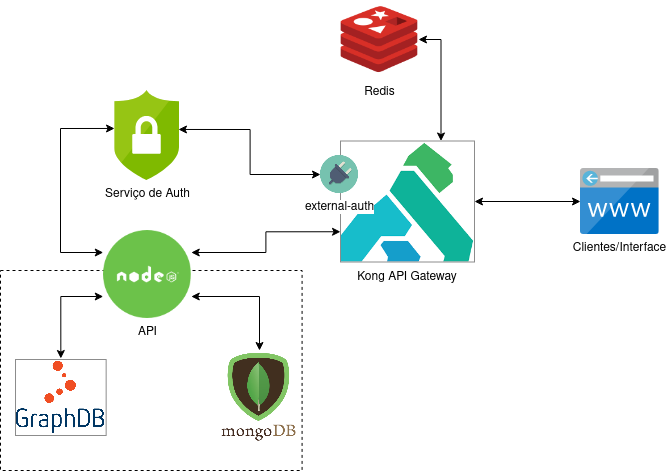
\includegraphics[width=0.9\textwidth]{img/apiGatewayArchFinal.png}
    \caption{Arquitetura desenvolvida com \textit{\acrshort{api} Gateway}}\label{fig:apiGatewayArchFinal}
\end{figure}

\section{Resumo}

De forma resumida, na secção do estado da arte foi descrito o que é uma \textit{\acrshort{api} Gateway} e seus objetivos bem como várias alternativas para a sua implementação existentes no mercado.

Já na secção da solução são descritos os requisitos necessários na plataforma \acrshort{clav}, escolhendo a alternativa que melhor se adequa.

A criação de uma \textit{\acrshort{api} Gateway} na \acrshort{clav} tem como principal intuito a simplificação da autenticação/proteção da \acrshort{api} de dados pelo que são considerados os requisitos mais apropriados a esta situação.

Finalmente, na secção da implementação, descrevem-se os passos realizados (desenvolvimento e configuração) para implementar a \textit{\acrshort{api} Gateway} e apresenta-se a arquitetura final desenvolvida.
